\documentclass{template/openetcs_report}
% Use the option "nocc" if the document is not licensed under Creative Commons
%\documentclass[nocc]{template/openetcs_article}
\usepackage{lipsum,url}
\usepackage{supertabular}
\usepackage{multirow}
\usepackage{color, colortbl}
\definecolor{gray}{rgb}{0.8,0.8,0.8}
\usepackage[modulo]{lineno}
\graphicspath{{./template/}{.}{./images/}}

\begin{document}
\frontmatter
\project{openETCS}

%Please do not change anything above this line
%============================
% The document metadata is defined below

%assign a report number here
\reportnum{OETCS/WP4/D4.2.3V10}

%define your workpackage here
\wp{Work-Package 4: ``Validation \& Verification Strategy''}

%set a title here
\title{openETCS Hazard and Risk Analysis and Safety Case Methodology}

%set a subtitle here
\subtitle{Overall methodology for the safety related activities to the openETCS on-board unit software development}

%set the date of the report here
\date{February 2015} %\\ Revised March 2013}

%document approval
%define the name and affiliation of the people involved in the documents approbation here
\creatorname{Jan Welte]}
\creatoraffil{TU Braunschweig}

\techassessorname{Abdelnasir Mohamed}
\techassessoraffil{AEbt}

\qualityassessorname{?}
\qualityassessoraffil{SQS}

\approvalname{Klaus-R\"udiger Hase}
\approvalaffil{DB Netz}

%define a list of authors and their affiliation here

\author{Jan Welte}

\affiliation{Technische Universität Braunschweig\\
  Institute for Traffic Safety and Automation Engineering\\
  Hermann-Blenk-Str. 42\\
  38108 Braunschweig, Germany\\
  eMail: openetcs@iva.ing.tu-bs.de \\
  WebSite: www.iva.ing.tu-bs.de}
  
  
\author{Merlin Pokam}

\affiliation{AEbt Angewandte Eisenbahntechnik GmbH\\
  Adam-Klein-Str. 26 \\
  90429 Nürnberg , Germany\\
  eMail: merlin.pokam@aebt.de \\
  WebSite: www.aebt.de}  

%add yourself as author, if you contributed to the document



% define the coverart
\coverart[width=350pt]{openETCS_EUPL}

%define the type of report
\reporttype{Output Document}


\begin{abstract}
This document describes the overall concepts for hazard and risk analysis and for the development of the resulting safety case as it has been identified during the first iteration of WP 4.
After the introduction defining the overall context of the document, the combination of methods is presented to identify hazards inside the openETCS software and to assess the risk resulting from these hazards for the system and subsystems. The sequence of activities is detailed on the proof of concept performed during the first WP 4 iteration. In the second part of this document the plan for the openETCS safety case is described. This includes the compilation of documents resulting from the performed openETCS software development as well as the derivation of a generic safety case structure for the development of a ETCS on-board unit using the openETCS software development process.
\end{abstract}

%=============================
%Do not change the next three lines
\maketitle
\tableofcontents
\listoffiguresandtables
\newpage
%=============================

\chapter{Document Control}

\begin{tabular}{|p{4.4cm}|p{8.7cm}|}
\hline
\multicolumn{2}{|c|}{Document information} \\
\hline
Work Package &  WP4  \\
Deliverable ID & D 4.2.3\\
\hline
Document title & openETCS Hazard and Risk Analysis and Safety Case Methodology \\
Document version & 01.0 \\
Document authors (org.)  & Jan Welte (TU-BS) and Merlin Pokam (AEbt)\\
\hline
\end{tabular}

\begin{tabular}{|p{4.4cm}|p{8.7cm}|}
\hline
\multicolumn{2}{|c|}{Review information} \\
\hline
Last version reviewed & 00.2 \\
\hline
Main reviewers (org.) & Olivier Hervillard	(Systerel), Hardi Hunger (DLR), Stephan Jagusch (Aebt) and Marielle Petit-Doche (Systerel) \\
\hline
\end{tabular}

\begin{tabular}{|p{2.2cm}|p{4cm}|p{4cm}|p{2cm}|}
\hline
\multicolumn{4}{|c|}{Approbation} \\
\hline
  &  Name & Role & Date   \\
\hline  
Written by    &  Jan Welte & WP4-T4.4 Task Leader  &  February 2015\\
\hline
Approved by & -- & -- & \\
\hline
\end{tabular}

\begin{tabular}{|p{2.2cm}|p{2cm}|p{3cm}|p{5cm}|}
\hline
\multicolumn{4}{|c|}{Document evolution} \\
\hline
Version &  Date & Author(s) & Justification  \\
\hline
00.0 & 01/10/2013 & Jan Welte &  Document creation \\
\hline  
00.1 & 28/01/2014 & Jan Welte &  Extended Introduction  \\
00.2 & 19/03/2014 & Jan Welte &  Reworded document structure to incorporate review comments from internal assessment \\
00.3 & 16/04/2014 & Jan Welte &  Incorporated Review comments \\
01.0 & 26/02/2015 & Jan Welte &  Incorporated new Design and changes in WP 3 work \\
\hline  
\end{tabular}
\newpage

% The actual document starts below this line
%=============================

\mainmatter

\chapter{Introduction}
\label{sec:introduction}

During system development the system limits and components have to be established before the necessary steps can be taken to ensure that the system behavior is not unsafe. In this context safety is understood as protecting humans from harm resulting from the system as distinguished from security which covers protecting the system itself from hazards coming from the outside. Respectively, safety and security are comparative terms which have to be specified in context of the system for which they shall be proven. With respect to the definition of safety used in the EN 50128 hazards are only taken in account with respect to direct harm to humans, not to the environment overall, as it is considered in other contexts. The standards for system development like EN 50126, EN 50128 and EN 50129 provide only guidelines how safety for a system shall be determined and assured by providing certain management principles and methods for the respective system development. As the openETCS project is related to a number of different system definitions like the overall railway system, the on-board unit, the Kernel software and the development tool chain different safety aspects have to be taken in consideration. Only a small number of these can actually be determined in the openETCS context alone. Respectively, this document and all considerations concerning safety in openETCS are focusing on the principal functional safety of the openETCS software and principals which have to be applied if the resulting model and software code shall be used in a specific context.

\section{Purpose}
\label{sec:purpose}

The hazard and risk analysis activities are part of the overall safety process which is defined in the EN 50129 as "the series of procedures that are followed to enable all safety requirements of a product to be identified and met". To ensure that the safety process is implemented in a proper way the EN 50129 requires a safety management which is consistent process for RAMS presented in the EN 50126. To do this the management has to present and control all related activities and documentations over the life-cycle taking into account the approval mile-stones and review requirements. As the product life-cycle is an ongoing process and iterative changes are taking place, the management system has to ensure that the respective safety effects of every change is considered. As the openETCS project does not cover the full development of an ETCS on-board unit, the safety related activities in WP 4 do not cover all required parts of a EN 50129 complaint safety process and management. Hence, the purpose of this document is to present the basic concepts for hazard and risk analysis and safety case development evaluated and derived during the first iteration of WP 4. As openETCS constitutes a research project planning and responsibilities can not be derived and confined as it would be expected in a pure development project. Respectively, this document is not intended to document all required roles, documents and responsibilities as it would be required for safety documentation according to EN 50126 and EN 50129. This report only intends to present concepts and principals which would fit the needs for openETCS and how these have to be applied up to this point in the project.

As the movement characteristics of a train set specific limits in which a driver alone is able to avoid derailment or any kind of collisions railway signaling and protection systems have been developed to ensure safe train movements. Respectively, the mayor parts of a train control system like ETCS include functionalities which shall guarantee that the overall railway system does not get in a hazardous situation. Correspondingly, this document illustrates the concepts for hazard and risk analysis which has been defined during the first WP 4 iteration to identify hazards or allocate them from the overall system analysis if they are related to the openETCS software. In addition the resulting risk for these hazards has to be evaluated to deduce specific safety requirements which have to be considered during the development process to reduce the risk. To support the concept presentation the results of the first proof of concept activities performed during this iteration are presented in section \ref{sec:Proofofconcept}.

As the openETCS project does not produce an implemented train borne on-board system, the openETCS documents will not cover all specific software and hardware aspects which the EN 50129 requires for a sufficient safety case. Respectively, the openETCS results cannot be used without further work to demonstrate that a derived product using the openETCS kernel is compliant with all specified safety requirements. On this grounds during the first WP 4 iteration a model-based concept has been derive how the openETCS contributions have to be presented to at least solve as a basis for an on-board unit safety case. Therefore, all documents shall be related to a generic safety case for an EVC using the openETCS software development.

\section{Document Structure}
\label{sec:document-structure}

As the openETCS software development process and the respective tool chain are used in an iterative process this document only presents the current state of the openETCS safety related activities as it only presents the results of the first WP 4 iteration. Chapter \ref{sec:introduction} gives an introduction to the overall document providing the basic document information and listing all reference standards and openETCS deliverables. Additionally, section \ref{sec:Background} provides an introduction concerning the context of quality and safety as it is understood in this document.

As the hazard and risk analysis and all safety case activities are directly related to the overall development process, chapter \ref{sec:development-process} introduces the general steps of the openETCS development process and its interface to safety activities. In the following chapter \ref{sec:hazardandrisk} the concept for hazard and risk analysis during the openETCS development is presented. The fundamental safety principal for ETCS, which are the starting point for all openETCS specific activities, are described in section \ref{sec:ETCS-safety}.
The derived plan how hazard and risk analysis may be perfomred for the openETCS software development is specified in section \ref{sec:Proofofconcept} and evaluated in a first proof of concept work performed during the first WP 4 iteration. Chapter \ref{sec:safetycase} describes the plan to collect and establish the safety case related documentation for the openETCS development, which has to be usable by following projects. While section \ref{sec:safetycase-structure} states the principal requirements for the overall safety case activities, section \ref{sec:safetycase-model} presents the model-based approach planed for openETCS and the supporting tools, which shall be applied.

\section{Document Evolution}

This document is based on the results of the first iteration work of WP 4 and shall present the overall concept for hazard and risk analysis methods using during the openETCS development. All resulting changes and additional safety activities have to be maintained and documented according to the overall safety process in following iteration and will be documented in the respective following deliverables. 

The openETCS development plan presented in chapter \ref{sec:development-process} is based on the development plan as it is described in the current version of the Quality Assurance Plan and in WP 2 deliverables D2.3 and D2.4. As the development methods and processes are still evolving this document has to be adopted accordingly. Concrete methods to verify and validate safety relevant properties derived from the hazard control methods described in this document, will be specified in the Verification and Validation plan. Also the tools used to support those activities will be detailed in this plan.

\section{Reference Documents}
\label{sec:refdoc}

This document essentially refers to the following standards, ETCS specification documents and openETCS project documents.

\begin{itemize}
\item \textbf{ISO~9000} --- 12/2005 --- \emph{Quality management}
\item \textbf{ISO~9001} --- 12/2008 --- \emph{Quality management systems — Requirements}
\item \textbf{ISO~25010} --- 03/2011 --- \emph{Systems and software engineering -- Systems and software Quality Requirements and Evaluation (SQuaRE) -- System and software quality models}
\item \textbf{CENELEC EN~50126-1} --- 01/2000 --- \emph{Railways applications –- The specification and 
demonstration of Reliability, Availability, Maintenability and Safety (RAMS) –- Part 1: 
Basic requirements and generic process}
\item \textbf{CENELEC EN~50128} --- 10/2011 --- \emph{Railway applications -- Communication, signalling and 
processing systems -- Software for railway control and protection systems}
\item \textbf{CENELEC EN~50129} --- 05/2003 --- \emph{Railway applications –- Communication, signalling and 
processing systems –- Safety related electronic systems for signalling}
\item \textbf{CCS~TSI} --- \emph{ CCS TSI for HS and CR transeuropean rail has been adopted by a Commission Decision 2012/88/EU on the 25th January 2012}
\item \textbf{SUBSET-026} 3.3.0 --- \emph{System Requirement Specification}
\item \textbf{SUBSET-091} 3.2.0 --- \emph{Safety Requirements for the Technical Interoperability
of ETCS in Levels 1 \& 2}
\item \textbf{SUBSET-088} 2.3.0 --- \emph{ETCS Application Levels 1 \& 2 - Safety Analysis}
\item \textbf{FPP} --- \emph{Project Outline Full Project Proposal Annex OpenETCS} -- v2.2
\item \textbf{D2.2} -- Report on CENELEC standard
\item \textbf{D2.3} -- Definition of the overall process for the formal description of ETCS and the rail system it works in 
\item \textbf{D2.4} -- Definition of the methods used to perform the formal description
\end{itemize}


%%%%%%%%%%%%%%%%%%%%%%%%%%%%%%%%%%%%%%%%%%%%%%%%%%%%%%%%%%%%%%%

\section{Glossary}
\label{sec:glossary}



\begin{tabular}{rl}
\textbf{ACedit} & Assurance Case Editor \\ 
\textbf{ARM} & Argumentation  Metamodel \\ 
\textbf{FMEA} & Failure Mode Effect Analysis \\ 
\textbf{GSN} & Goal Structured Notation \\ 
\textbf{MoRC} & Management of Radio Communication \\ 
\textbf{SIL} & Safety Integrity Level \\ 
\textbf{SRS} & System Requirement Specification \\ 
\textbf{THR} & Tolerable Hazard Rate \\ 
\textbf{V\&V} & Verification \& Validation \\ 
\end{tabular} 




\section{Background Information}
\label{sec:Background}

As safety is a term which is used in different contexts and therefore interpreted differently depending on the used reference system, the following section \ref{sec:Background} presents the principal concept and terminology on which the following safety process is founded. Thereby, this section mainly bases on the understanding of safety as it is used in standards EN~50126, EN~50128 and EN~50129 for railway system development. In the context of railway system development the EN~5012X and the ISO~900X standards are closely connected. Respectively, the terms safety and quality and related terms as reliability, maintainability, availability, usability and security are often used together. For example the EN~50129 names evidence of quality and safety management as conditions for a safety acceptance. The following sections shall give a common definition for all this aspects, which are required in a CENELEC confirm development process. 

\subsection{Quality}

The ISO~9000 defines quality as "degree to which a set of inherent characteristics fulfills requirements", which clearly shows a more objective view as the EN~50129, which defines quality as "a user perception of the attributes of a product". As for system development the given requirements always present the objective against which the system has to be measured this definition is consistent with the definition of verification and validation as it is presented in the EN~50128 and the openETCS Verification and Validation plan.

Depending on the respective field of application specific standards further specify the characteristics which shall be taken in account to establish quality. The EN~50126 as primary standard for railway applications gives RAMS as the major contributor for the quality of service. 

\subsection{Software Quality}

The ISO~25010 for software engineering defines quality of a system as "the result of the quality of the system elements and their interaction" and therefore separates between two different so called quality models for software. Software quality covers the local software specific quality aspects by defining eight software characteristics: functional, suitability, reliability, performance efficiency, operability, security, compatibility, maintainability and transferability (see figure \ref{fig:Software-Product-Quality-eng}).

\begin{figure}[htbp]
\centering
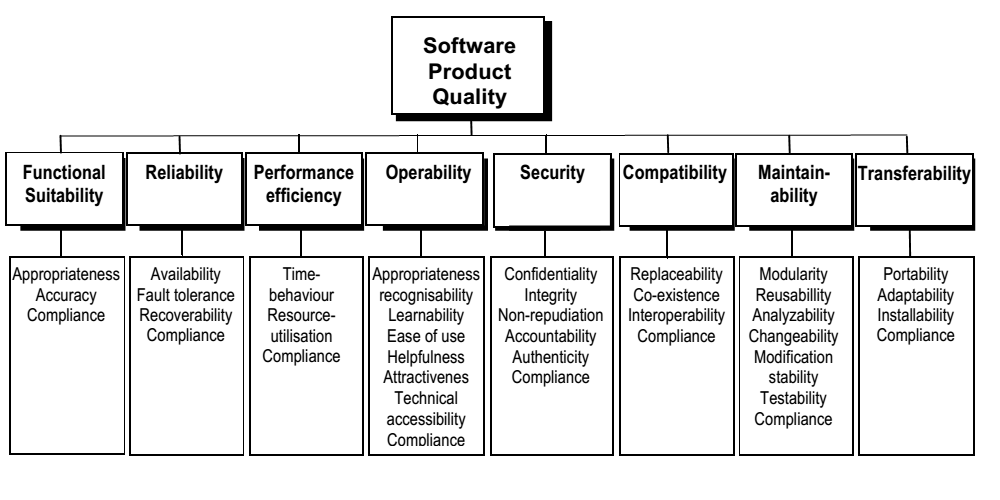
\includegraphics[width=0.8\linewidth]{Software-Product-Quality-eng}
\caption{Software Product Quality as defined in ISO~25010}
\label{fig:Software-Product-Quality-eng}
\end{figure}


These can be assess for software itself independently of the operational  context for which the software has been developed. On the other hand the quality in use model represents those characteristics measuring quality related to the operational environment in which a specific user applies the software. The standard defines here three characteristics: 
usability in use, flexibility in use and safety in use (see figure \ref{fig:Software-Quality-in-use}).

\begin{figure}[htbp]
\centering
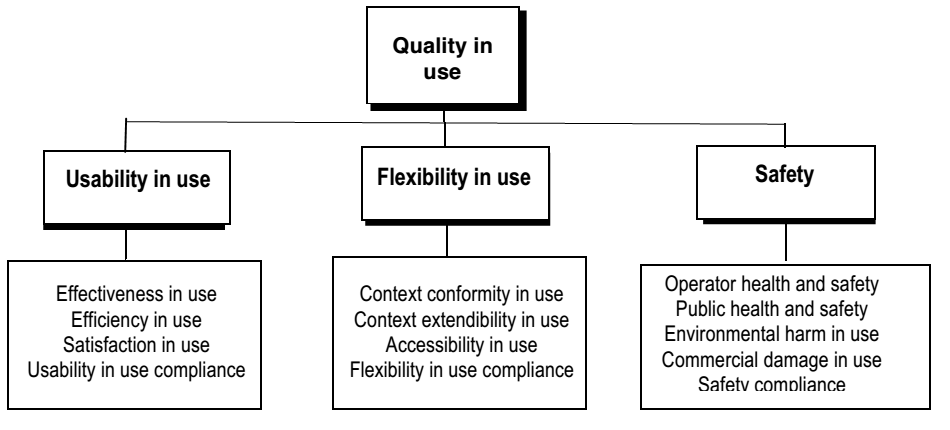
\includegraphics[width=0.7\linewidth]{Software-Quality-in-use}
\caption{Software Quality in use as defined in ISO~25010}
\label{fig:Software-Quality-in-use}
\end{figure}

This distinction between local and system quality characteristics shows that functional correctness and safety is closely related for a safety relevant system, but with respect to the development these have to be addressed different to evaluate their quality.

\subsection{Railway RAMS}

Safety in the railway development as defined in the EN~50126 is in considered in the over all context of Quality of Service and the specific relations between reliability, availability, maintainability and safety, short RAMS. These aspects represent the major contributions to the overall quality of service and have to be evaluated throughout the whole life cycle.

As represented in figure \ref{fig:RAMS-EN50126} reliability and maintainability are characteristics which can be applied to the local system as these are specific to the application of this system. In contrast availability and safety are global characteristics as both depend on the behavior and dependences between different components of the overall system.

\begin{figure}[htbp]
\centering
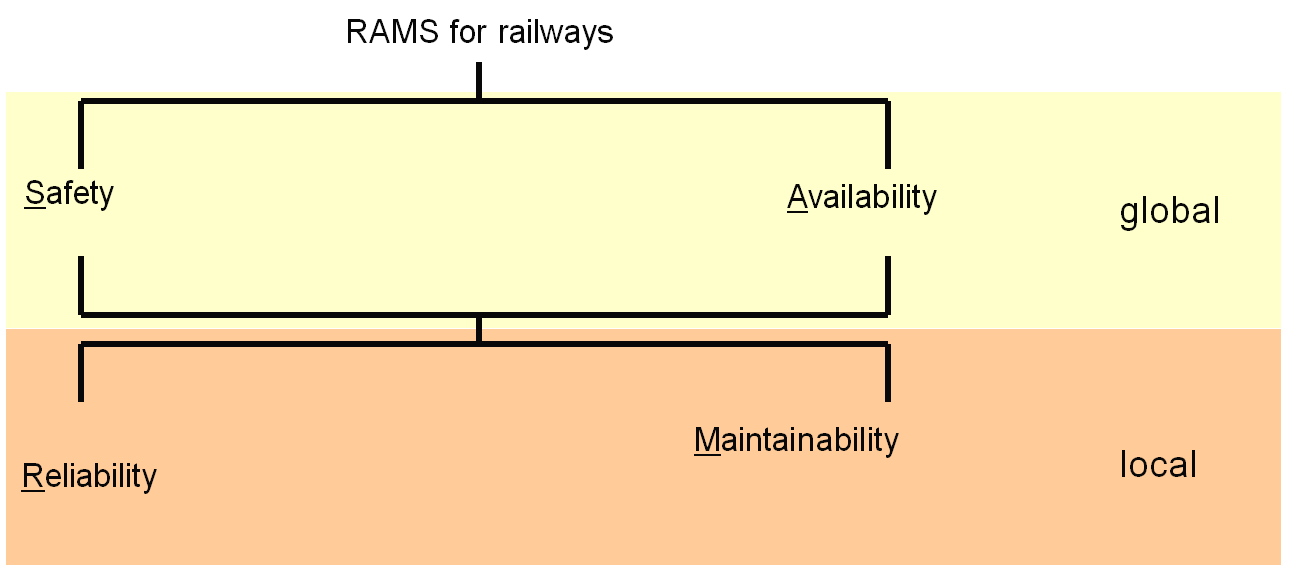
\includegraphics[width=0.7\linewidth]{images/bld_RAMS-Railway-50126}
\caption{RAMS for Railway elements and their relations \cite{Schnieder.2013}}
\label{fig:RAMS-EN50126}
\end{figure}

These dependences between the local and global system characteristics and the static and dynamic system aspects are shown in figure \ref{fig:Reliability-RAMS}. 

\begin{figure}[htbp]
\centering
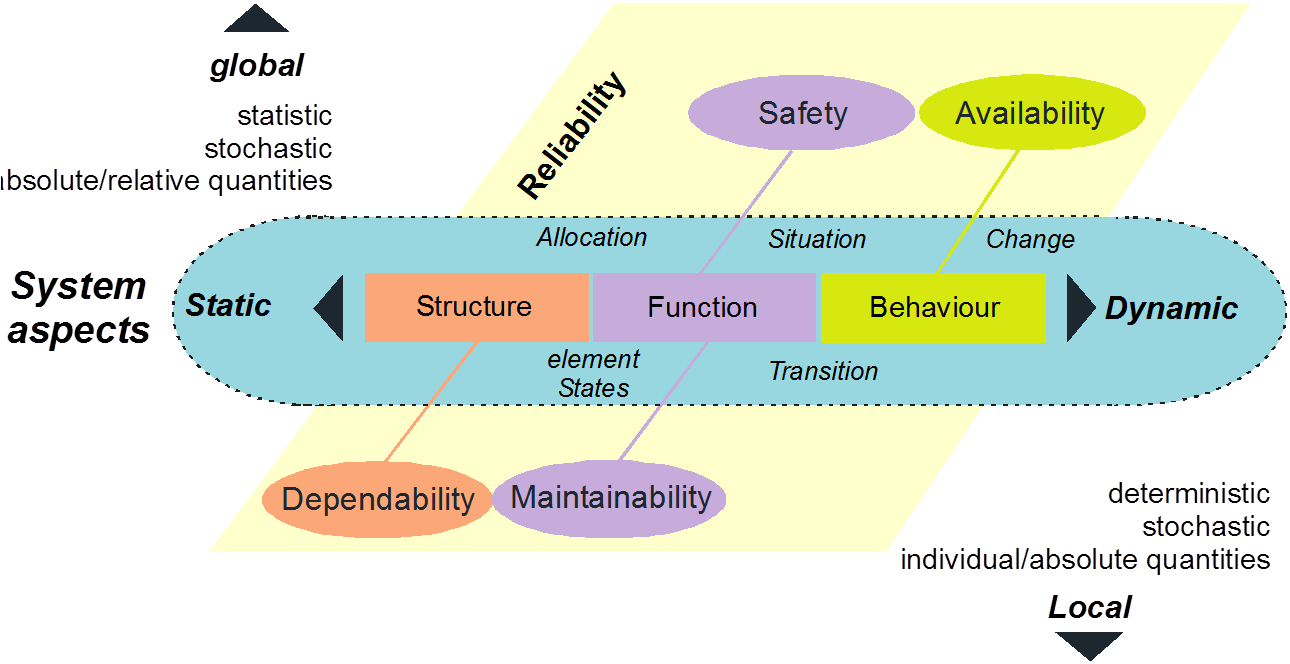
\includegraphics[width=0.7\linewidth]{images/bld_Reliability-system-characteristics}
\caption{Systems Characteristics and their relations to RAMS in Railways \cite{Schnieder.2013}}
\label{fig:Reliability-RAMS}
\end{figure}


\subsection{Probabilistic Functional Safety Concept}

The EN~50128 standard defines safety as the ``freedom from unacceptable levels of risk of harm to people", which shows that the safety approach required by the CENELEC standards is risk-based.

\paragraph{Risk}

 As the risk is defined as the ``combination of the rate of occurrence of accidents and incidents resulting in harm (caused by a hazard) and the degree of severity  of that harm" in the EN 50128 this approach is based on a probabilistic understanding of event occurrence. The overall relations between all these safety-related terms used to define the safety properties, characteristics and quantities are outlined by the Risk-Genesis-Model of Schnieder, which is shown in the following figure \ref{fig:Risiko-Genese-Modell-eng} \cite{Schnieder.2010}.

\begin{figure}[htbp]
\centering
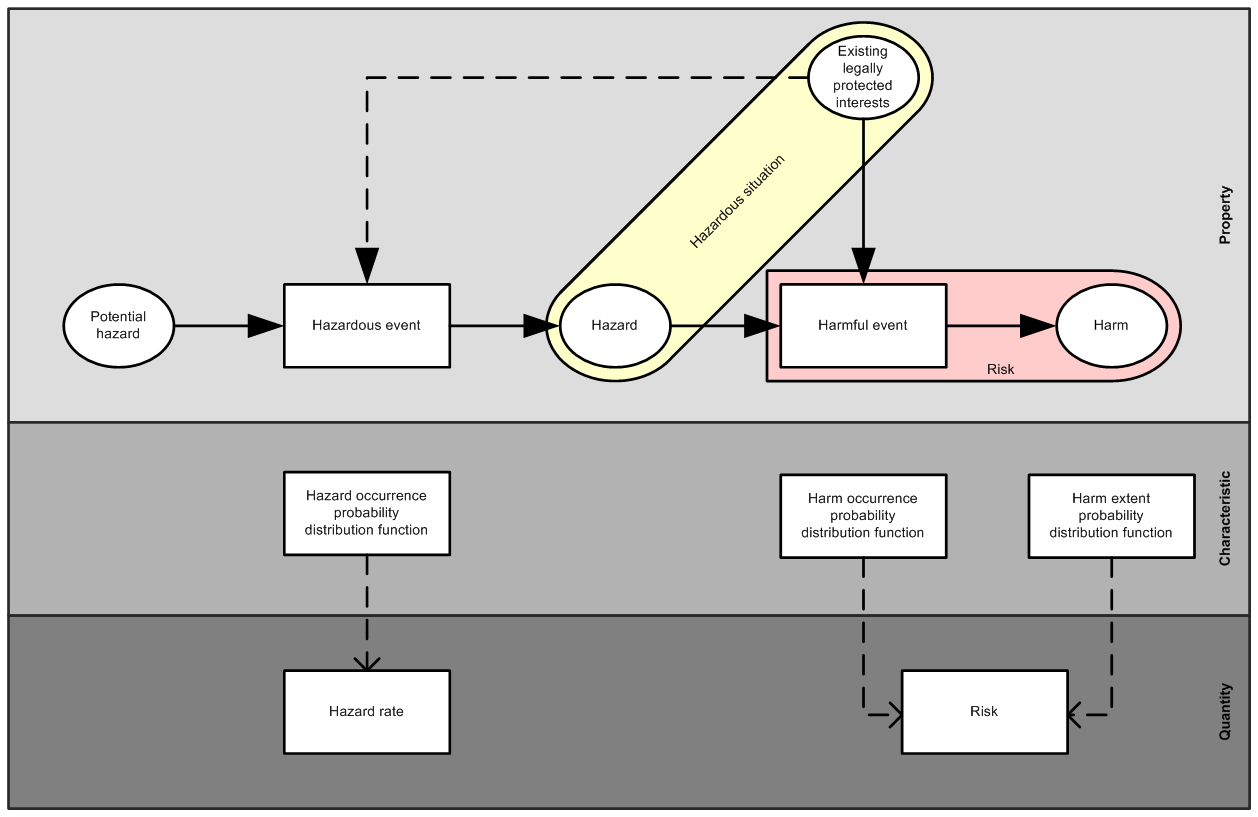
\includegraphics[width=0.8\linewidth]{bld_2013-06-19_Risiko-Genese-Modell-eng-2-0_jw}
\caption{Risk-Genesis-Model showing the relations between the safety-related terms \cite{Schnieder.2010}}
\label{fig:Risiko-Genese-Modell-eng}
\end{figure}

This demonstrates that for every specific hazardous situation a harmful event can be identified which will result in harm. The probability of occurrence for this event combined with the probable extent of harm is defined as risk.

\subsection{Hazard and Risk Analysis}
\label{sec:HandR-Ana}

Based on the probabilistic safety concept the first step to evaluate the existing risk is to define the system properties, specifically identifying the harms and their related hazardous situations. This has to be performed during a system hazard analysis. Afterwards the respective properties have to be determined by assessing the risk concerning the identified hazards. Respectively, a risk analysis and assessment is defined in the ISO/IEC Guide 51 as a systematic use of available information to identify hazards and to estimate the risk. The EN 50129 states a hazard analysis as the process of identifying hazards and analysing their causes, and the derivation of requirements to limit the likelihood and consequences of hazards to a tolerable level. This extends the ISO/IEC Guide 51 definition by adding a risk reduction. As this demonstrates that the terms hazard and risk analysis are used synonymous to represent the respective process, containing the following tasks, to reduce risks to a tolerable level:

\begin{enumerate}
\item identify the likely users for the product or system including vulnerable consumers; 
\item identify the intended use and assess the reasonably foreseeable misuse of the product or system; 
\item identify each hazard (including reasonably foreseeable hazardous situations and events) arising in the stages and conditions for the use of the product or system including installation, maintenance, repair and destruction/disposal; 
\item estimate and evaluate the risk to the affected user group arising from the hazard(s) identified;
\item if the risk is not tolerable, reduce the risk until it becomes tolerable.
\end{enumerate}

Accordingly, the hazard and risk analysis represents an iterative process of risk reduction and risk assessment carried out repeatedly until the risk in the system could be sufficiently reduced. The general iterative process to achieve the acceptable risk according to ISO/IEC Guide 51 is shown in figure \ref{fig:risk-analysis}.

\begin{figure}[htbp]
\centering
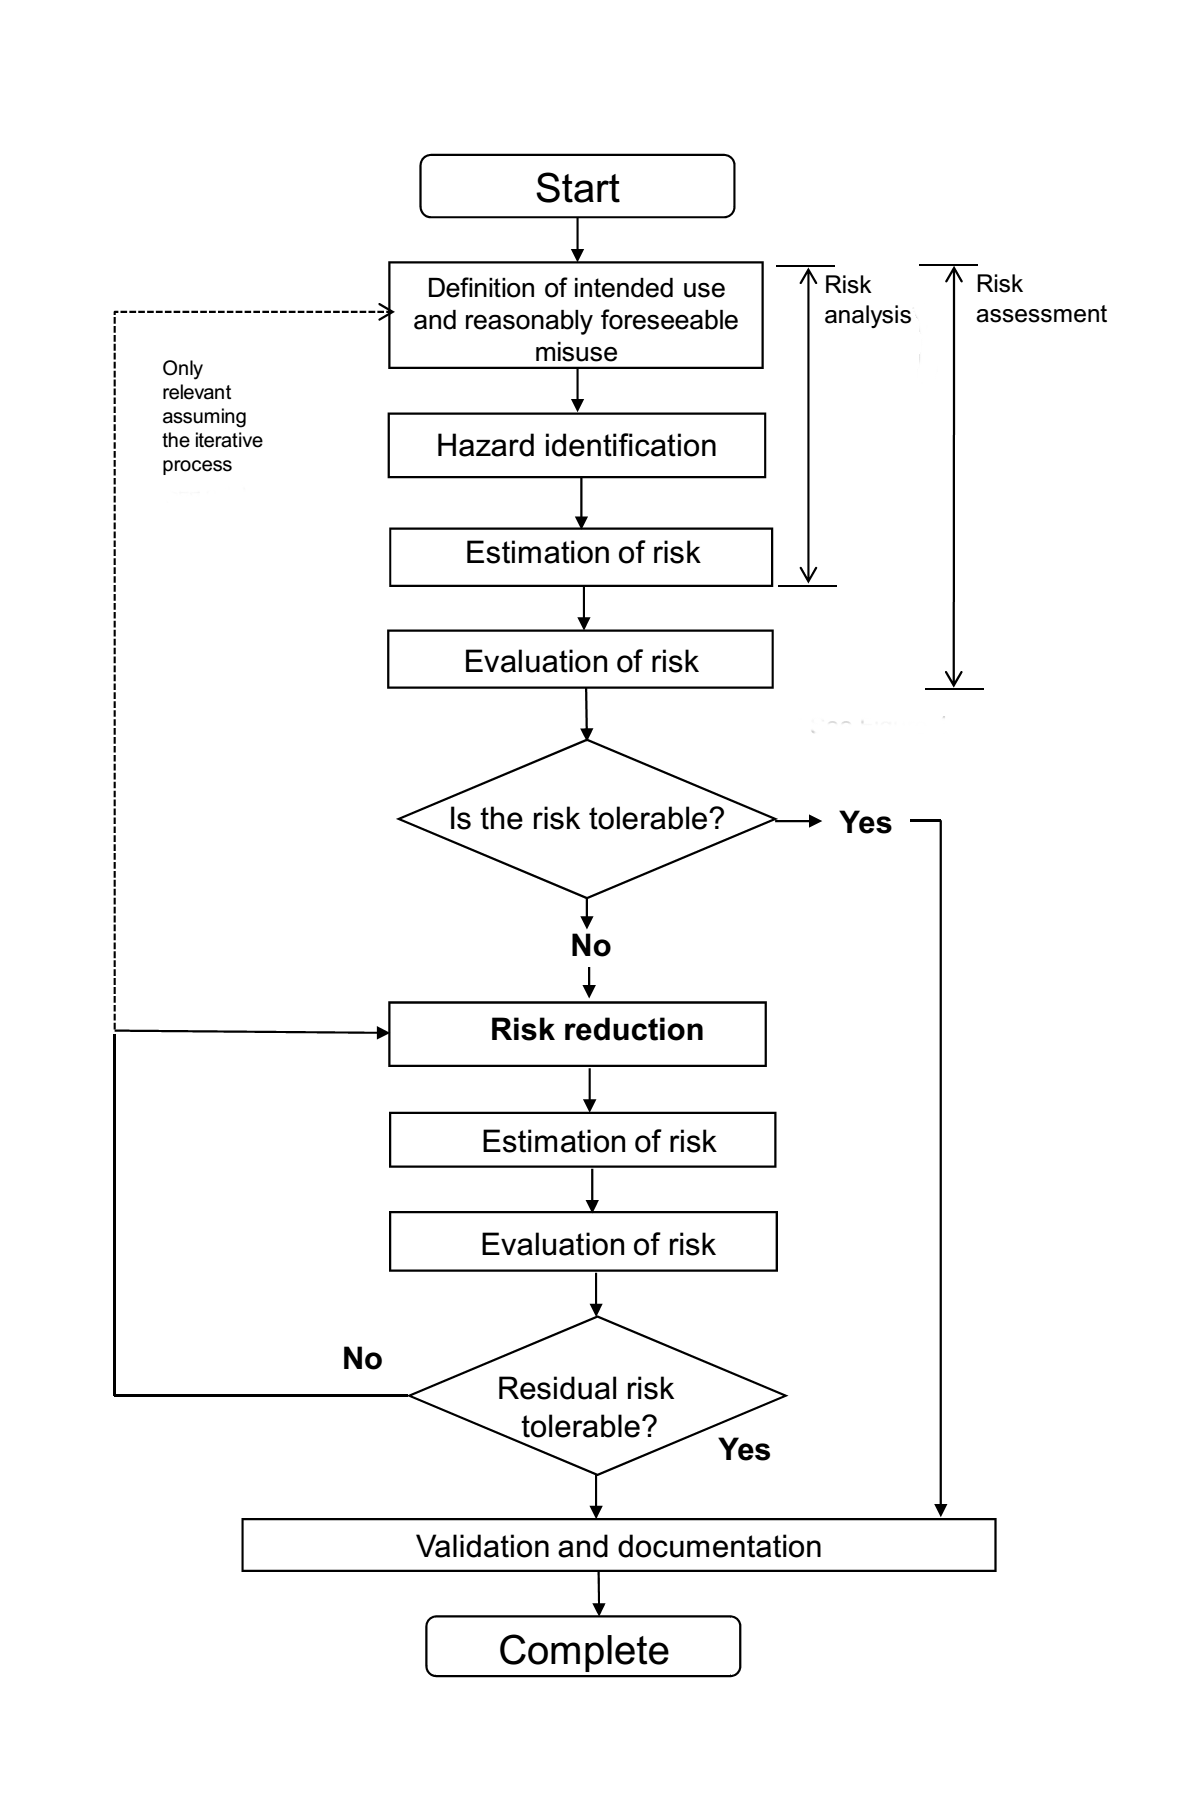
\includegraphics[width=0.6\linewidth]{ISO-Guide-51-risk-analysis-and-assessment}
\caption{Risk analysis and assessment process in ISO-Guide-51}
\label{fig:risk-analysis}
\end{figure}

\subsection{Safety Integrity Level}

Since risk, due to  uncertainty in real systems and to its multidimensional nature, cannot be eliminated completely, it is necessary for risk reduction to identify a relative level  as the required level of safety for a system. This is the accepted risk, which is classified under the operating conditions of the system to be sufficiently low and thus be acceptable. The safety integrity level (SIL) represented the acceptable risk for every part of the system. The risk control process as it is presented in figure \ref{fig:Risk-control-modell-eng} is then performed to ensure that the safety integrity levels are reach by every part of the system.

\begin{figure}[htbp]
\centering
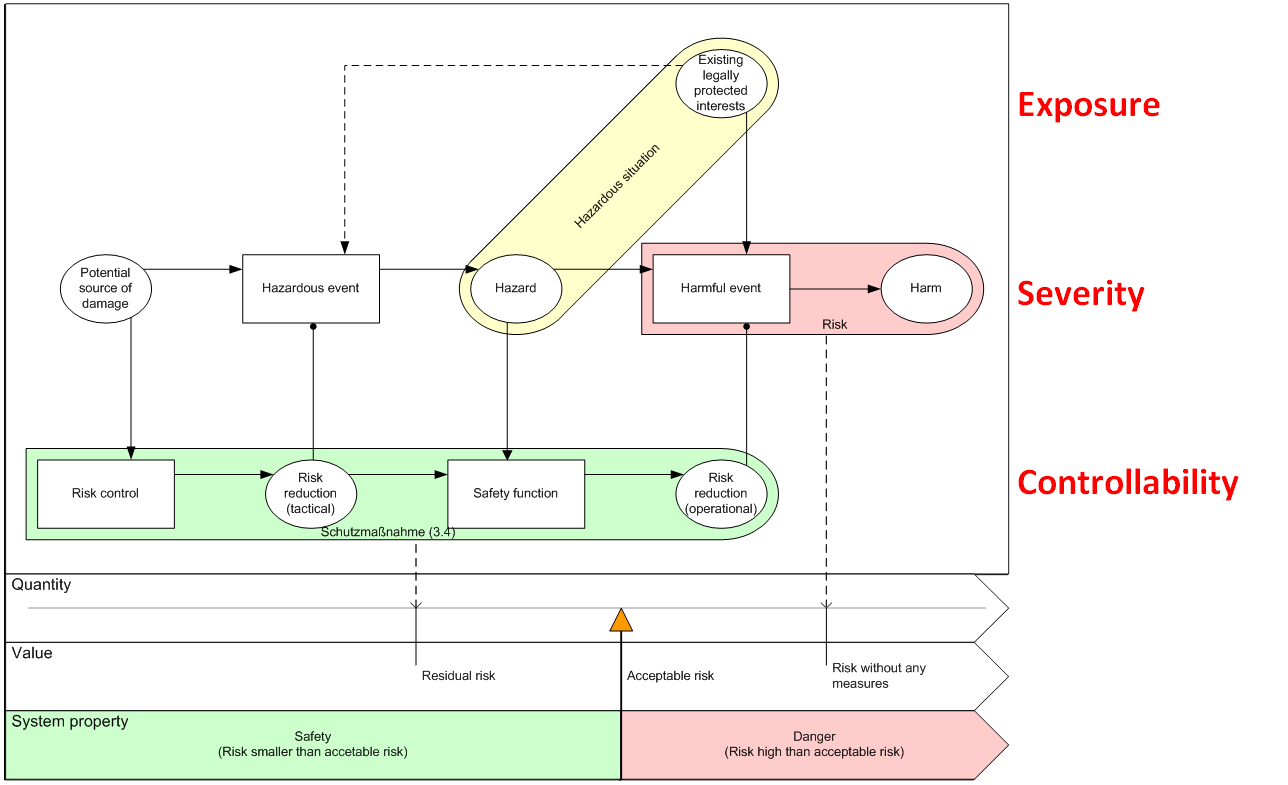
\includegraphics[width=0.9\linewidth]{bld_2013-06-19_Risk-control-modell_1-0_jw}
\caption{Risk control process \cite{Schnieder.2013}}
\label{fig:Risk-control-modell-eng}
\end{figure}

Since software itself does not fail in the way technical equipment fails, the specific software safety integrity level can be better understood as a qualitative measure with respect to the required degree of correctness for the software functionality than as a quantitative value for the likelihood of failing. To reach the needed degree of correctness for the software various design, verification and validation methods are required corresponding to the assigned software safety integrity level. This process leads to safety requirements which have to be implemented in the software design as well as verified and validated. Respectively the EN~50126 describes the safety design process as a series of safety tasks for each life cycle phase. This task are related to a number of safety artifacts which are created, used and adapted over time through the different safety design activities.

\subsection{Safety Case}

The EN~50129 states that evidence of quality management, safety management, as well as functional and technical safety have to be provided for safety acceptance. The safety case shall be the structured safety justification document demonstrating that these conditions have been satisfied.
Therefore, the British Ministry of Defence defines a safety case as “a structured argument, supported by a body of evidence that provides a compelling, comprehensible and valid case that a system is safe for a given application in a given environment.”\cite{MinistryofDefence.2007} This definition emphasizes the distinction between the “argumentation” and the “evidences”, which corresponds to the distinction between rules coming from the legal requirements and facts resulting from the actual working process. This clear distinction between the safety argumentation and the evidences helps to structure the safety case and improvement of the discussions with the legal authorities.\cite{Muller.2010}

%\subsection{Safety Glossary}

%\textbf{Added via the glossary documentation process for openETCS}



\chapter{OpenETCS Development Process}
\label{sec:development-process}

The main products of the openETCS project will be the openETCS specification model used to generate the openETCS on-board software and the openETCS tool chain development, which is used to formalize the ERA Specifications for ETCS, generate the Software Code and perform verification and validation activities. Both parts have their own development process, but the focus for the hazard and risk analysis and the safety case shall be on the software development process. The openETCS tool chain shall only be considered with respect to its role in the software development process as the openETCS project spends the effort to provide a qualifiable tool chain, but will not be able to provide all evidence for a complete qualification.

\section{Formalization and Software Development}

The software development in the OpenETCS project shall be performed as an open, model-based, agile Software development using the SCRUM methodology. The respective combination of methods used during the development process shall comply with a SIL 4 development process according to EN~50128 for which the requirements are analyzed and shown in detail in D2.2. The overall OpenETCS Software development process presenting the development principles are outlined in WP 2 D2.3 and D2.4. Accordingly, the on-board unit requirements for ETCS shall be extracted from all ETCS system documents. These are mainly the SUBSET 26  and for specific parts further parts of the TSI CCS Annex A. In context of the EN 50128 development the the ETCS specification managed by the ERA mainly SUBSET 26 represents the basis for System Requirement Specifications and System Architecture Description. Nevertheless, those documents have to be adopted to derive the Requirement Specifications for the openETCS on-board Software. Based on these requirements specifications, which will be specified using the tool ProR by creating various ReqIf Requirement Specification files, the following work will be done using different model-based approaches. Software Architecture and Design will be documented by a formalized Software Architecture Model as a SysML  model. Afterwards the Software Design and Software Interfaces will be documented in detail by a formal SCADE behavior model, which is in an agile way process combined from a number of component Design Models in SCADE. Respectively Software and Component Design are a combination of top-down and bottom-up work in a congenerous model environment to ensure component integration. As the integrated SCADE model is the basis for the automatic source code generation the functional integration will be performed exclusively during the SCADE component model integration. Only wrapper parts shall be integrated on source code level. All supporting documentation is generated directly or with main support by the model-based tool-chain.

Figure \ref{fig:DevopmentProcess} shows the general artifacts for the openETCS Software development mapped to the EN~50128 V-model development life cycle. As the Verification and Validation activities are specific to the design artifacts further details are not available at this point. The Verification and Validation plan describes a number of methods which can be applied for different properties in the context of the openETCS development principals.

\begin{figure}[htbp]
\centering
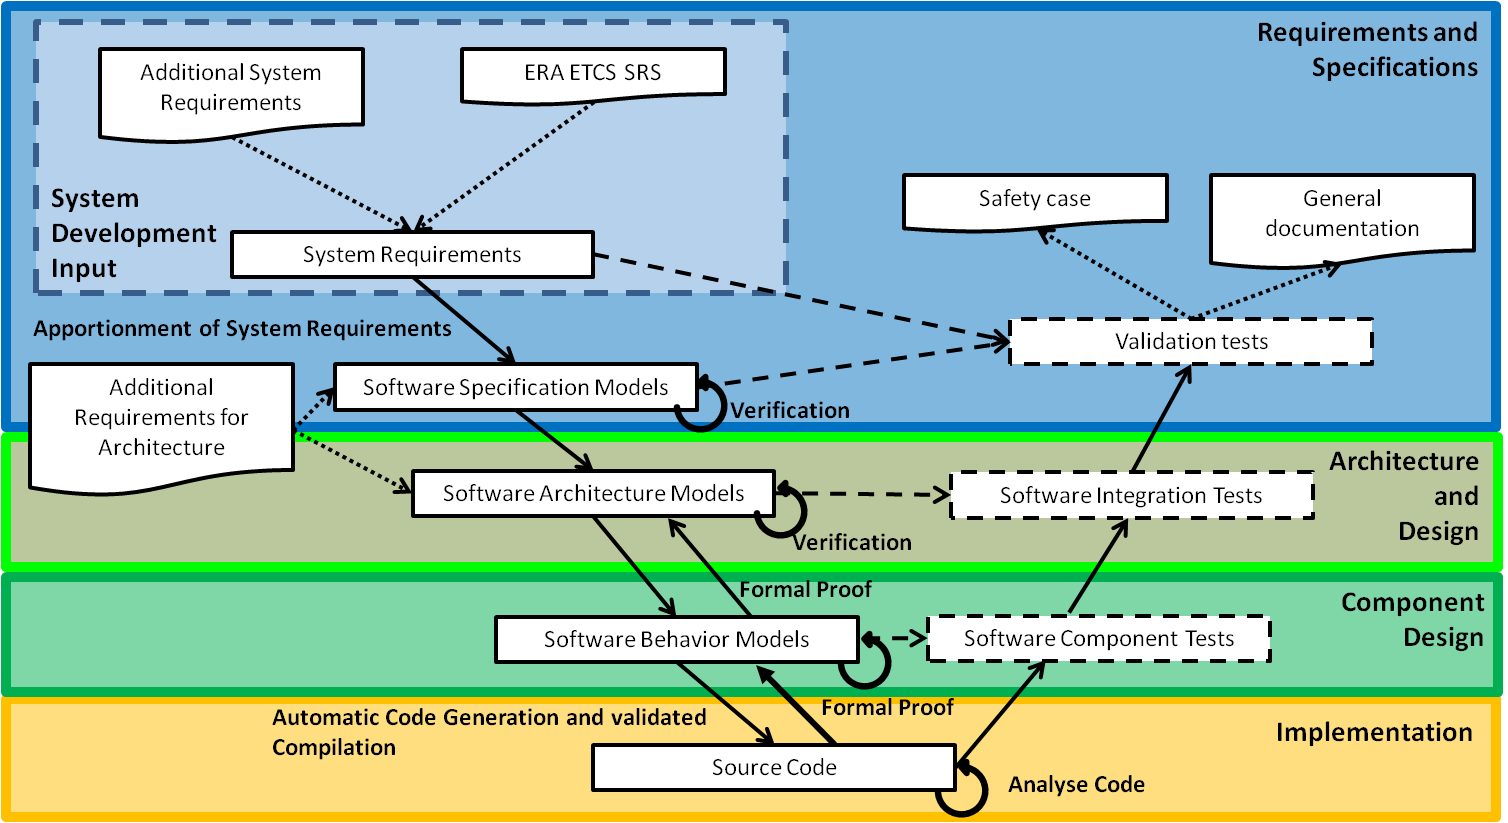
\includegraphics[width=1.0\linewidth]{./images/openETCS-Software-Development_2-0}
\caption{Overall openETCS software development process}
\label{fig:DevopmentProcess}
\end{figure}

The detailed principals and phases of this development process including all related artifacts and used tools have to be presented in the Quality Assurance Plan.  As the project continues this development process and the supporting tools are still evolving, respectively the detailed development description has to be updated in the Quality Assurance Plan continuously.

Corresponding to the development artifacts the openETCS development process has 5 main distinguishable phases show in table \ref{tab:DevelopmentPhases}. Every phase besides the validation phase is mostly supported by one means of description and one corresponding tool, but the overall traceability of the development requires linking requirements and design elements between all phases. 

\begin{table}[htbp]
  \centering
  
  \caption{Phases openETCS software development process}
\begin{tabular}{|p{1cm}|p{2cm}|p{7.5cm}|p{2.5cm}|}
\hline \textbf{Phase} & \textbf{Name} & \textbf{Description} & \textbf{Main Tool component} \\ 
\hline P1 & Software Requirement Phase & Requirement input documents converted to a ReqIF format and informally analyses. The analysis specifies relationships between requirements and revises parts of the requirements to obtain a detail and atomic abstraction level usable for moralization. To support thus the requirements are categorized and grouped. & ProR \\ 
\hline P2 & Software Architecture Modeling Phase & Building a SysML based on the informal analysis using the categorization of requirements. The architecture model focuses on functional blocks and data flows. & SysML Papyrus \\ 
\hline P3 & Software Behavior Modeling and Integration Phase & Building the SCADE model for the separated basic functional blocks. The SCADE model describes the detailed behavior for the function using the data flows. & SCADE Suite \\ 
\hline P4 & Code Generation Phase & Based on the SCADE Behavior Model C code will be automatically generated. This C code is than compiled to executable code which runs on the EVC. & SCADE Suite + C Code compiler\\
\hline P5 & Formal Validation Phase & Using test models and model checking techniques, to validate the correct model behavior.  & Various tools \\ 
\hline 
\end{tabular} 
\label{tab:DevelopmentPhases}
\end{table}

The phase P1 Software Requirement Phase covers the development activities required by the EN~50128 during its lifecycle phase Software Requirements Phase (7.2). The SUBSET 26 and further System Specifications are the Input of this work. The resulting ReqIF Requirement file shall represents the Software Requirement Specifications. The Software Overall Test Specification will be derived with respect to this, but a method is not defined at this point.

The phase P2 Software Architecture Modeling Phase and P3 Software Behavior Modeling and Integration Phase cover activities of Software Arch. \& Design Phase (7.3), Software Component Design Phase (7.4) and Software Component Implementation Phase (7.5) by the EN~50128 development lifecycle. The SysML model represents the Software Architecture Specifications and a first version of Software Interface Specifications. The Output SysML model is in the following phase transformed into a SCADE model which will be refined and enhanced to completely represent Design and Interface Specifications as well as all Component Design Specifications. As the overall SCADE model is composed of serveral compoent SCADE models and the defined interfaces the integration is performed and documented in the SCADE model. Input for all architecture and design tasks are the Software Requirement Specifications based on the SUBSET 26. Source Code in C is generated automatically via the certified SCADE Code Generator and combined with required wrapper software. For these wrapper parts specific development methods have to be defined as these parts are specified.

The phase P5 Formal Validation Phase has to cover activities of the Software Component Testing Phase (7.5), Integration Phase (7.6) and mainly Software Validation Phase (7.7) by using simulation, testing and model checking methods already available in the SCADE environment as well as additional tools. The Input for these activities are the SysML and SCADE models and the C Code.

Although the phase represent different working steps in the life cycle according to EN~50128 the agile development process applied in openETCS induces that the phases are performed iteratively during the development process. Respectively, the traceability linking in combination with the verification methods has to ensure that changes in one phase of the development are adopted for all linked artifacts up- and downwards in the development process.

\section{Interfaces to Safety Activities}

As safety is a system property the software development has to be performed according to the safety functionalities allocated to the software. Thereby, the resulting Software SIL defines the combination of quality methods to be performed to ensure that all requirements including the allocated system safety requirements are implemented correctly. To provide all needed justification that the required Software SIL is reached, the development has provide complete documentation for the safety case. As the openETCS software development is not part of a specific system development, but has the objective to specify and implement the overall ETCS functionality, it has to interact with a respective generic safety management process and take the overall safety requirements for a train control system into account. As show in figure \ref{fig:SafetyProcess} the over all development is determined by a number of interactions between design, verification and validation and the general quality and safety management.

\begin{figure}[htbp]
\centering
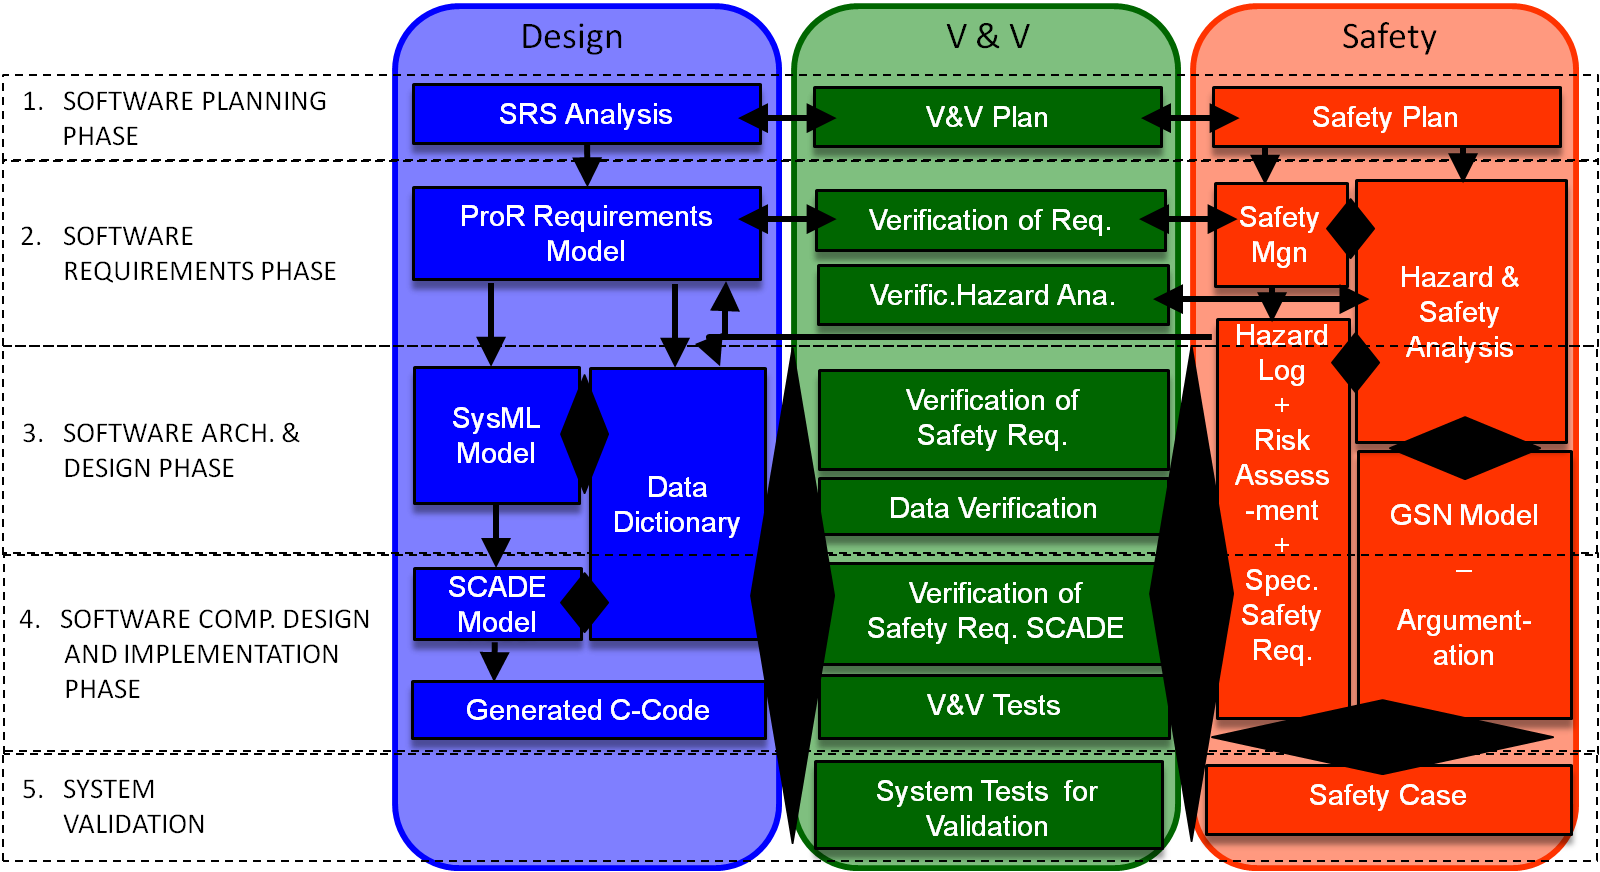
\includegraphics[width=1\linewidth]{./images/openETCS-Software-Safety-Development}
\caption{OpenETCS development relations between design, verification and validation and safety activities}
\label{fig:SafetyProcess}
\end{figure}


\subsection{Interface to Quality and Safety Management}

In parallel to the design process the safety management process has to perform hazard and risk analysis methods for the software design to ensure that the design concept can reach the expected safety integrity level for the overall system. Thereby, potential hazards resulting from the software functionality and its design have to be identified and their risk has to be assess in the system context. To control the risk respective measures have to be taken, which be realized through additional safety requirements to which the design has to be conform. The hazard log represents the central element of this safety management as it collects the hazards and manages the respective risk control.

As the Software SIL determines the development methods which have to be applied to ensure a correct development, the quality management has to ensure that these methods are chosen according to the standard and are applied correctly. This has to be specified in the Quality Assurance Plan and to be documented in the overall safety case. 

\subsection{Specific Interfaces to the Design Process}

To be able to respect the system safety requirement these have to be apportioned to the different software components. This has to be done for all abstraction levels during the system design. 

\subsection{Interface to Verification and Validation}

Design verification activities will ensure that all system requirements including the safety requirements have been apportioned and implemented correctly at the respective software component. Software validation will ensure that the overall software implementation matches all specified requirements which implicates requirements derived from the hazard and risk analysis. To do so all requirements concerning SIL and SSIL development level and their respective accepted risk have to be taken into account in a hazard and risk analysis process. The resulting risk reduction tasks have to be represented as explicit technical specifications. The process requirements resulting from SSIL level have to be incorporated in the quality assurance process. In addition it has to be verified that all hazard and risk analysis methods as well as the methods for assembling the safety case have been chosen and applied appropriately. This has to be done against the methodology requirements specified in the Quality Assurance Plan and further referenced documentation as a safety plan.
Respectively, the verification and validation plan shall specify the appropriate methods for these design and implementation verification and validation activities. All resulting reports are evidence for the qualified software development and become part of the safety case.



\chapter{Hazard and Risk Analysis}
\label{sec:hazardandrisk}

As presented in subsection \ref{sec:HandR-Ana} hazard and risk analysis are required to identify hazards, estimated and evaluate the resulting risk for the assumable use of the design object. This respective risk has to be evaluated against an acceptable risk level determined based on use and context of the system and its environment. If the risk exceeds the acceptable level risk reduction steps have to be incorporated until an acceptable level can be reach conclusively. 

This chapter presents a basic concept how those activities shall to be addresses during the openETCS project activities and which results are provided in this way to support the development and further use of openETCS results. 

\section{Risk Analysis in Context of EN 50126}
\label{sec:EN50126-risk-analysis}
The EN 50126 as main norm for the RAMS system development of railway applications uses in subsection 4.6 the term risk analysis to introduce the general concept of hazard identification and risk reduction as it has been detailed in subsection \ref{sec:HandR-Ana}. Thereby, the standard clearly states that the concept of assigning SIL levels to components of a system can only be done in context of the system risk analysis, as the hazard propagation can only be considered through the overall system structure. 

\subsection{Purpose and Scope}

The EN 50126 establishes the risk analysis as phase 3 of the system lifecycle during which a System Hazard and Safety Risk Analysis shall be performed. This shall establish the Hazard Log to collect all identified hazards and their respective analysis and a respective risk assessment. The standard clear states risk analysis has to be repeated at various points during the system development to accommodate for refinements and changes done in the following lifecycle phases. 

Respectively, the purpose of risk assessment is to provide detailed analysis for hazards and resulting risk arising from the system - in case of openETCS the ETCS on-board kernel software -  in its operational environment. Risk control measures have to be established and refined at more detailed during the development phases to ensure that the existing risk is limited to an acceptable level. 

\subsection{Objectives}

For the risk analysis lifecycle phase the EN 50126 states the following objectives to be achieved on system level:
\begin{enumerate}
\item identify hazards associated with the system.
\item identify the events leading to the hazards.
\item determine the risk associated with the hazards.
\item establish a process for on-going risk management.
\end{enumerate}

The fourth point basically requiring the continuous risk analysis process which has to be established on the beginning of system development and to be refined over the lifecycle and for component development. Hereby, the Hazard Log is the central deliverable by recording all hazard related information , their respective risks assessment and taken control measures. These information have to be considered and extended with all key inputs from subsequent lifecycle phases.

\subsection{Activities}

To fulfill the requirements for a risk management process as stated in EN 50126 methods and tools for the following activities have to chosen and applied:

\begin{itemize}
\item establishing a Hazard Log and continuously manage it over time
\item identifying hazardous situations on various levels
\item estimate consequences and frequencies associated with each identified hazardous situation
\item calculate risk these hazardous situations and their respective combinations
\item estimate the acceptable risk for the system and its various components
\item identify and evaluate control measures to reduce or eliminate the risk for these hazardous situations
\item continuously reevaluate refine and reevaluate hazardous situations, risk and control measures
\item document results, assumptions and limits for all activities performed
\end{itemize}

All these activities have to be done considering quality and change management processes and the results have to be verified according to the general rules. A wide range of methods for hazard and risk analysis exists and examples like the risk graphs, severity matrices, FTA or FMEA are common and used for different activities.


\section{Plan Hazard and Risk Analysis for openETCS}

The safety design process and the resulting documentation constitute the main documents for the system approval, as it is required by European and national law to do everything reasonable expectable to prevent harm. Accordingly the CENELEC standards build the common technical rules for the development process. The Common Safety Methods present a concept based on the EN50126 how the risk evaluation and management has to be performed. 

Therefore the main references concerning the safety design process are the CENELEC standards, mainly the EN50126 on how the safety aspects have to be handled as part of the RAMS management over the development process. The overall risk evaluation concept is also defined at this point. The specific concerning the safety case preparations are defined in the EN50129 including the Safety Integrity Level concept. 

\subsection{Purpose and Scope}

 Instantiation of 50126 process for openETCS
 
 - System and Specification 
    (Object of initial step of HRA, relevant specs)
 - identify later stages (as far as foreseeable)"
 
 Since the ETCS system specification for the on-board unit shall be formalized and implemented in the software during the openETCS software development, the specific safety requirements for the on-board unit have to be determined according to the overall system requirements. These are mainly given by the following two parts of the CCS TSI:
 
 \begin{itemize}
 \item UNISIG SUBSET-026	System Requirements Specification 	(Version 3.3.0)
 \item UNISIG SUBSET-091 Safety Requirements for the Technical Interoperability of ETCS in Levels 1 and 2 	(Version 3.2.0)
 \end{itemize}
 
 In relation to SUBSET-91 further documents should be take into account to derive specify safety aspect:
 
 \begin{itemize}
 \item Part of TSI Annex A
 	\begin{itemize}
 	\item SUBSET-036
 	\item SUBSET-037
 	\item SUBSET-040
 	\item SUBSET-041
 	\item SUBSET-098
 	\end{itemize}
 	
 \item Not part of TSI Annex A
 	\begin{itemize}
 	\item SUBSET-039
 	\item SUBSET-078
 	\item SUBSET-079
 	\item SUBSET-080
 	\item SUBSET-081
 	\item SUBSET-088
 	\end{itemize}
 \end{itemize}
 

\subsection{Objectives}

\label{sec:ETCS-safety}

Based on the ETCS reference architecture SUBSET-91 gives the role of ETCS as train protection as the following:

\begin{center}
\textbf{"To provide the Driver with information to allow  him to drive the train safely and to enforce respect of this information, to the extent advised to ETCS."}
\end{center}

Respectively, the Core Hazard for the ETCS reference architecture is defined as the following in SUBSET-91:
\begin{center}
\textbf{"Exceedance of the safe speed or distance as advised to ETCS."}
\end{center}

Based on the role of ETCS and its respective SIL 4 quantification the maximum allowed rate of occurrence (Tolerable hazard rate) of the ETCS Core Hazard for ETCS on-board is
\[1.0\times10^{-9} hour^{-1} train^{-1}.\]
The same value is specified for the corresponding track-side.

Adapted form the ETCS system safety analysis presented in SUBSET-88 the Annex A of SUBSET-91 presents the List of Hazardous Events inside ETCS that might cause the ETCS Core Hazard to occur, either alone or in combination with other failures. These are the events not eliminated by the operational analysis. 34 of these hazardous events are allocated to the Kernel, which make them the basis for the on-board software hazard and risk analysis. 

\subsection{Activities}

Based on these overall safety goals as specific hazard and risk analysis for the software subsystem has to be performed to allocate the requirements and set-up the openETCS hazard log as shown in figure \ref{fig:SafetyProcess}. Cased on the principle software architecture the risk can be assess, which then leads to the definition of risk control measures. These are the basis for specific safety requirements for the on-board unit software design and its verification and validation. During the development these requirements are adopted if necessary for the different abstraction levels from the high level model down to the source code. The safety case, which shall be supported by a Goal Structured Notation (GSN) \cite{GSNwebsite} model as presented in chapter \ref{sec:safetycase} has to present all needed documentation to show that these leads to the required risk level.

The openETCS hazard and risk analysis covers the relevant activities presented in section \ref{sec:EN50126-risk-analysis} at least in a way to demonstrate that the model-based openETCS development process is sufficient to support all required activities to comply to EN 50128 SSIL 4. As the development process is still not specified in all a details this document can only present a concept and has to be enhance during the ongoing work.

\textbf{Hazard Log}

The Hazard Log as the central artifact for the hazard and risk control will be established and managed as a structured list via the github document management system as all openETCS artifact to ensure version and configuration management. The artifact will include the list of all identified hazards and their relations as well as derived risk assessment and control measures. To provide the complete documentation links to the detailed analysis documents will be include as well as for required V\&V reports. Doing so the changes will be managed by issues as only the core commiters for V\&V are managing the artifact. 

\textbf{Identifying Hazardous Situations and Estimation of Consequences and Frequencies}

The analysis to identify hazards and hazardous situations will be addressed via a combination of top-down and bottom-up analysis. The top-down analysis will be performed by FTA based on the system analysis presented in SUBSET-88 and SUBSET-91. Thereby, only measure concerning the actual software functionality and the development can be applied in the openETCS context. Constraints for the hardware implementation have to be provided as for further use.
Based on the openETCS Architecture partners will apply model based FMEA and -if applicable - HAZOP analysis as bottom-up approach. 

Hazard consequences and occurrence will be evaluated based on the FTA and FMEA results. As openETCS mainly deals with functionality specified by the software most hazards have to be circumvented completely. This has to be done throughout a structured analysis performed by a group of different stakeholders from system, design and V\&V.

\textbf{Risk Calculation and Evaluation}

A qualitative risk evaluation will be performed by Frequency - Consequence Matrix. As quantitative risk calculations are based on operational circumstances, which can change for ETCS on-board units due to different operator procedures, the openETCS activities can only use generic quantitative values provided by via ERA system evaluations. The same limitation has to be stated for the implementation, as the risk calculation can only use assumptions for hardware, but is not able to use any specific information.

\textbf{Identifying and Evaluating Control Measures}

As openETCS mainly deals with control software, which shall exhibit a deterministic behavior, the control measure will mainly be derived by creating boundaries to avoid conditions under which the system reaches the unsafe state. The main measures to ensure this will be to ensure data consistence for the cycle calculation process used and forcing the software functions to go into fail safe states if unexpected or inconsistent inputs are received. 

\textbf{Documentation}

The hazard Log as the central artifact will provide the relations for all documents and ensure completeness for a related documents. These will be provided by the responsible partner for respective analysis and as far as possible generated by the respective tool. All documents have to follow the review and quality process of openETCS.

\section{Summary of Proof of Concept}
\label{sec:Proofofconcept}

To evaluate the hazard and risk analysis process in the openETCS development environment a proof of concept has been performed during the VnV Level 1 activities in WP 4 by project partners Systerel, All4Tec and AEbt. As the respective design artifact for the proof of concept a SysML modeled formalizing one part of SUBSET-26 has been chosen: 

\begin{center}
\textbf{"\S 3.5 Management of Radio Communication (MoRC)."}
\end{center}

This model has been created by the project partner Siemens during the design process first in SCADE and then extended to a SysML model. The Model can be found under \url{https://github.com/openETCS/model-evaluation/tree/master/model/SCADE_Siemens/MoRC_System/MoRC_System/SysML_Model}. For the Proof of Concept only the SysML model has been used as the scope was on the hazard and risk analysis for the SysML architecture allocation.

To do so the following hazardous event given in SUBSET-91 has been identified as the event mainly related to this part of the specification:
\begin{center}
\textbf{“KERNEL-6 Manage communication session failure” which results an “RADIO (INFILL) Transmission data consistency failure (safety related transmission function)”.}
\end{center}

The following task have been performed during the Proof of Concept as examples for the activities during a hazard and risk analysis. The first part represents the basic verification needed for the assess functionality models. The second part represents hazard identification with respect to the core hazard and the related harm. The derivation of safety targets represents the risk calculation an evaluation for the identified functions. Respective control measures are presented by all derived safety requirements.
The third part then demonstrates the check and evaluation of these general control measures for the specific model under review.
 
\begin{enumerate}
\item Conformity comparison for the MoRC
	\begin{itemize}
	\item Conformity comparison regarding sub functions between SUBSET-26 and SysML model
	\item Conformity comparison regarding Input and Output data between SUBSET-26 and SysML model
	\end{itemize}
	
\item Safety Analysis for the MoRC
	\begin{itemize}
	\item Hazard \& Risk analysis for each sub functions
	\item Derivation of safety Target (SIL) for each sub functions
	\item Derivation of safety requirements for each sub functions
	\end{itemize}
	
\item Safety Assessment for the MoRC
	\begin{itemize}
	\item Derivation of the safety requirements
	\item Assessment of the model against these safety requirements
	\end{itemize}
\end{enumerate} 
 

The first task conformity comparison has been performed to verify the model, as no formal verification process has already been performed on the chosen preliminary model. The conformity was passed, as all sub function of the subset 026 function (MoRC) and those of the model match together and all Input \& Output data for each sub function of the subset 026 function and those of the model also match together. 

 
The second task Safety Analysis was performed using methods for three different safety activities as defined in the EN~50129 standard: hazard identification,
risk estimation and evaluation, derivation of the Safety requirements. In general hazard identification and risk analysis are performed using traditional approaches like FMECA or HAZOP. In the case of openETCS since models are available a model-based, computer supported approach (based on the Tool “Safety Architect” from the company ALL4TEC) for hazard identification has been used in addition.
Both results have been compared at the end to validate the results.
 
For functions coming from the Subset 026 a hazard and rick analysis has been already performed, including a SIL allocation as presented in Subset 091. All these functions have a SIL 4 safety requirement; therefore sub function from these functions shall also a SIL 4 safety requirement. For functions and corresponding sub function coming from others sources than the SUBSET-26 a SIL allocation on the basis of techniques described in the standards EN~50126, 50129 or IEC 61508-5 shall be performed.
 
The third Task of the process consists in performing a Safety Assessment, which implies derivation of safety requirements and the following assessment of the model against these safety requirements. The derivation of the Safety requirements required knowledge in the function being analyzed, the interfaced components, the ETCS in general and CENELEC standard.
  
The details results for the Proof of Concept can be found at \url{https://github.com/openETCS/validation/tree/master/VnVUserStories/VnVUserStoryAll4Tec-AEbt}. 

The safety requirements issued from this analysis have been formally specified and proved on an Event-B model by Systerel. The resulting models and documents are available at \url{https://github.com/openETCS/validation/blob/master/VnVUserStories/VnVUserStorySysterel/04-Results/d-EventB-VnV/EventB-Rodin-VnV.pdf}.

Overall the Proof of Concept has confirmed the correctness of the model as far as this has been possible in the limited scope. 

The FMEA has identified 23 hazardous events in the subsystem which could lead to the Kernel 6 event. As measure to prevent this occurrence of these events 18 safety criteria have been derived.  

The model-based safety analysis showed 12 safety assumptions related to over 40 granular function events. These are related to the assumed unwanted behavior in different subfunction blocks. Overall both methods seam to create comparable results, but due to the status of the model and the complexity of the mathematical model-based analysis both results are difficult to match. Respectively, the model-based analysis has to be specified further to fit the modeling process. But due to the size of SUBSET-26 on-board function, the model-based analysis is in the focus to lower the amount of manual work.
 
As the proof of concept has clear shown that the process is able to derive Safety requirements, which can be allocated to different specification based on the software architecture, the results can be used to define the openETCS hazard and risk analysis process.
 
\section{Hazard and risk analysis supporting tools}

Supporting software tools are needed to handle the safety artifacts and to some degree to more efficiently perform the safety design activities. As some safety artifacts like the safety requirement specifications and the safety backlogs are closely related to design artifacts the same tools can be used. Especially all requirements should be handled by one tool to ensure full traceability and provide one main interface for the verification and validation activities.

Depending on the methods used for hazard and risk analysis appropriate tools are needed to perform the analysis, collect the hazards and associated risks in the hazard log and to evaluated possible risk control measures. Thereby, traceability has to be guaranteed between all activities. As the main architecture will be designed in SysML, safety analysis tools like the Safety Architect Tool will be used to analyze the hazard propagation in the functional decomposition and to derive the resulting risk level. In this way short feedback iterations to the design process can be realized.

\chapter{OpenETCS Safety Case}
\label{sec:safetycase}

In general the safety case has to present to the assessing authority that the development has be done according to the required standards and that the product confirms to the quality and safety level corresponding to the aspired utilization. 
To do so the present chain of argumentation has to state the requirements for the product development, its derived specifications and the evidence that the work has been done accordingly. To do this the safety case has to collect and combine documents from many different activities during the work process. As these documents are usually produced and stored in different places and formats studies have shown that a large amount of time to produce the safety case is spent on searching for document, maintaining document contents and maintaining document references \cite{Muller.2010}. 

\section{Structure}
\label{sec:safetycase-structure}
As the openETCS development has the objective to produce a reference formalization and implementation for the ETCS on-board unit, which can be used by interested parties during further development, it is highly important to collect all relevant documents in a way that fulfills the requirements for safety relevant system development. If thereby the distinction between basic assumptions, safety argumentation and evidences for the openETCS development is presented properly in the safety case the discussions with the legal authorities is improved and reusability is made easier. 

Overall the openETCS will separate between the following three kind of evidence in compliance to the safety acceptance conditions stated in the EN~50129. 

\subsection{Quality Management Evidence}

Since the openETCS project as a research does not have the objective to conduct all steps needed for a vital on-board unit development, the resulting safety case will be generic in many parts only giving the requirements and basic safety strategies, but lacking the actual evidence. However, the overall safety argumentation has to be set up to meet SIL 4 requirements. Therefore the safety case has to show that the methods chosen in the openETCS development process satisfy the EN~50128 quality requirements and which documents have to be created during the process to obtain the required evidence. Basis for this work will be the Quality Assurance Plan, which builds the basis for all quality management activities.

\subsection{Safety Management Evidence}

As detailed in chapter \ref{sec:hazardandrisk} the overall safety argumentation has to demonstrate that during the development process the higher-level safety requirements have been addressed and that accordingly the on-board software satisfies the safety level. As this will be done using the basic process presented in chapter \ref{sec:hazardandrisk}, the safety case has to specify the traces from high-level hazardous events to all subsystem requirements allocated to the openETCS software architecture and their verification and validation. Therefore, the safety case has to present evidence that the chosen methods are sufficient to demonstrate compliance to the requirements and that they are applied in a consistent process which ensures that all safety requirements are respected and validated.


\subsection{Functional and Technical Safety Evidence}

The main evidence for this part will be the validation results which proof that the actual models and/or the code satisfies the overall safety principles. The generic safety case shall clearly state all specific artifacts to present for any adapter of the openETCS software which artifacts have to be provided by him and which content can be reused for his overall safety argumentation.

\section{Model-based Argumentation}
\label{sec:safetycase-model}

The openETCS safety case shall present a transparent and easy to understand argumentation chain referring to the relations between the sequential and parallel processes in the development process and the respective requirements in the normative EN~50129 safety case. Capitalize on the basic principles applied during the openETCS development the safety chase can be enhance by using a model-based representation connected to the central data base to reference the respected artifacts \cite{Muller.2010}. Thereby, the model provides a graphical representation of the argumentation chain, which makes it possible to directly identify in which development step which requirements is addressed and which are the respective artifacts containing the design and the corresponding evidence. 

In this way the generic safety case presents the over argumentation structure connecting requirements, design artifacts and evidence. The specific openETCS safety case is then provided trough the linking to the github data based providing document versions and status information to ensure consistence throughout the evolving documentation.

\subsection{Goal Structured Notation}

Interviews performed during the INESS project have shown that graphical argumentation structures ease the discussions between with legal authorities as it provides a look on the essence of the argumentation strategy in an easy way. During the method evaluation the Goal Structuring Notation (GSN) \cite{Kelly.2004thegoal, GSNwebsite} has been identified as suitable argumentation notation, already use in industrial projects, to  graphically  to model the relations between individual requirements, methods and evidence in a safety case. The argumentation demonstrates how each requirement will be address by a tree structure of derived subgoals and the resulting evidence to satisfy these goals as shown in figure \ref{fig:GSN-SafetyCase}. The different notes in the tree will be linked to the openETCS development artifacts in the github document management system. Additionally the artifacts will be linked to the modeled documentation of the EN~50128 development process during the corresponding phases to demonstrate the process conformity. 
 
\begin{figure}[htbp]
\centering
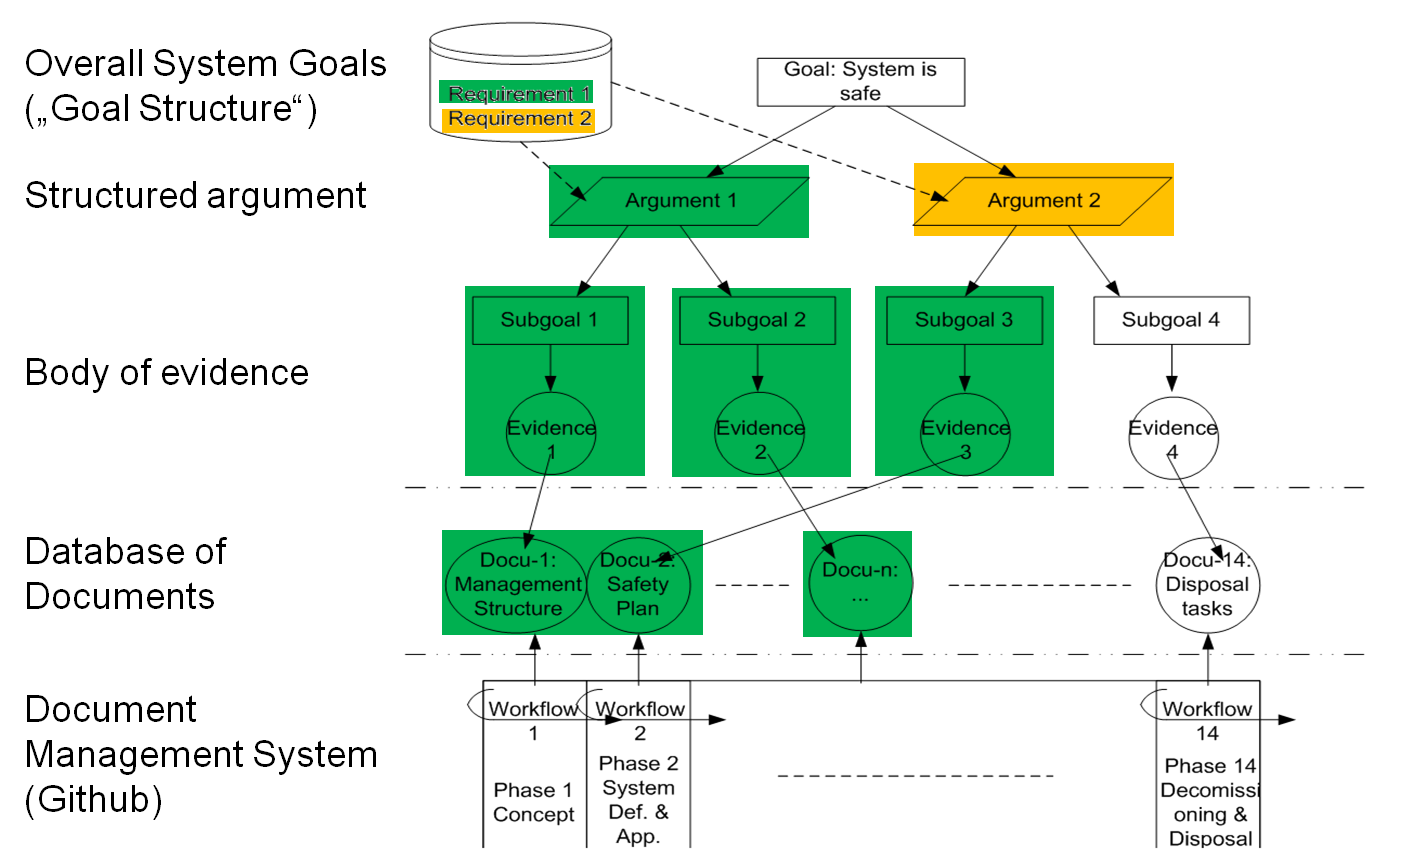
\includegraphics[width=0.9\linewidth]{./images/Structure-SC-GSN}
\caption{Structure model-based safety case using GSN}
\label{fig:GSN-SafetyCase}
\end{figure}

 In addition, the graphical model and its reference to the different artifacts provides as valuable option for external and internal parties to locate and retrieve the right information from the diverse data base structure of the opneETCS project.

\subsection{Safety Case Supporting Tools}

To support the proposed model-based safety case a safety case editor to model GSN argumentation structures is needed. For the artifact relations the editor has to provide an interface to connect individual model element to specific artifacts in the document management system. An ideal support for the automatic evolution of the safety case would be provide when the interface allows the exchange of meta data concerning the artifacts like status and version, which can be presented in the model to demonstrate the current status.

Since the openETCS development uses the eclipse tool platform and the github document management system as the backbones for the tool integration and the artifact management, the tool supporting this model-based safety case approach shall be able to interact with these two. 

The Assurance Case Editor (ACedit) \cite{aceditwebsite} is a tool implementation of GSN \cite{GSNwebsite} and the OMG Argumentation  Metamodel  (ARM) \cite{ARMwebsite} to graphically construct argumentation structures to which this tool refers as assurance cases. In addition the tool supports a number of model management techniques including model checking methods that apply to GSN and ARM. As ACedit is eclipse based the evaluation done during the verification and validation level one has determined this tool as the most promising GSN editor. Since the eclipse framework provides an interface to github via the EGit plug-in the document management system integration shall be realized through the eclipse model base.

The GSN editor developed during the INESS project has been dismissed as it is only java based. The effort needed to connect this tool to eclipse and github during the openETCS projet was sat as to high. 
 
\chapter{Conclusion}
\label{sec:conclusion}

This document has presents the basic concept for the main safety related activities in the openETCS development as they have been determined during the first verification and validation iteration level of WP 4. As these have been set in respect to a still evolving development methodology and tool chain, the overall process as to be detailed and adopted as the project continues. 

As the openETCS development presented in chapter \ref{sec:development-process} formalizes the SUBSET-26 requirements using SysML and later SCADE models, the hazard and risk analysis methodology applied at the openETCS development has to be able to allocate all hazardous events relevant for the kernel of the on-board unit to subsystems of the openETCS software architecture. Based on this allocation the resulting risk will be determined leading to safety requirements to control the overall system risk allowed level. 

The results for the proof of this concept conducted during the first verification and validation level by Systerel, All4Tec and AEbt using the benchmark SysML model for Management of Radio Communication and one allocated hazardous event has show that the proposed methodology for hazard and risk analysis provides sufficient safety requirements for the design process. Further specification of the methodology has to be done to support or even replace the manual FMECA or HAZOP with an automatic analysis of the SysML model by the Safety Architect tool. However, the proof of concept has demonstrated that this could be sufficient and the best option to work in short design iterations as the openETCS project plans to do. 

In general the verification and validation activities have to ensure that the safety principal apportioned to the on-board functionality are satisfied. Hence, the main objective for the openETCS safety case as presented in chapter \ref{sec:safetycase} is to provide the fundamental quality and safety principles for the openETCS development as these have to be completed by adopters of the openETCS results for their assessment. Therefore, the general safety argumentation and the concrete evidences shall be clear distinguished to ease applicability and support discussions with different legal authorities.

Modeling the generic argumentation structure and connecting the individual elements to the respective artifacts created during the openETCS development has been identified during the first level iteration as a promising approach to show the relations between requirements, safety strategy and provides evidence. A GSN model combined with direct links to the actual artifacts in the document management system should also help the internal and external discussions concerning the safety strategy. To efficiently use this approach for the safety case preparation the  chosen ACedit editor for GSN has to be interfaced with the github document management system. 

Overall the main methodology for the hazard and risk analysis as well as the safety case work has been defined during the first level iteration but these concepts have to be further refined over the next iterations with the evolving development process.

\bibliographystyle{unsrt}
\bibliography{./ref/ref-HaRA}


%===================================================
%Do NOT change anything below this line

\end{document}


